\subsection*{Efterbehandling}
Hvis vores eksperiment havde forløbet præcis,
som vi havde ønsket, så ville den noterede
masse af produkt være korrekt, dvs. $3{,}25\ \unit{\gram}$.
Desværre viste det sig, at svovlsyren, som vi brugte, slet ikke var svovlsyre,
det var nemlig saltsyre. Det har ikke betydet,
at reaktionen ikke kunne forløbet, tværtimod.
Det har dog betydet, at der har været saltsyre 
rester i vores produkt, da natriumcarbonat-opløsningen
skulle fjerne svovlsyren og ikke saltsyre.

Før vi begynder at vurdere, hvilken betydning
det så må have haft for ligevægten af reaktionen,
så kan vi lige udregne det teoretiske udbytte.
Her skal vi også have nogle overvejelser, vi antager,
at methanol er tilsat i overskud, som det også er,
så det ikke vil være en begrænsende faktor.
Derfor finder vi molarmassen for salicylsyre og
methylsalicylat:
\begin{align*}
    M(\ce{C6H6OHCOOH})&=138{,}12\ \unit{\gram/\mol} \\
    M(\ce{C6H6OHCOOCH3})&=152{,}14\ \unit{\gram/\mol}
\end{align*}

Nu kan vi udregne stofmængden af $\ce{C6H6OHCOOH}$:

\begin{align*}
    n(\ce{C6H6OHCOOH})&=\frac{m(\ce{C6H6OHCOOH})}{
        M(\ce{C6H6OHCOOH})
    }=\frac{8{,}99\ \unit{\gram}}{138{,}12\ \unit{\gram/\mol}}
    =6{,}51 \cdot 10^{-2}\ \unit{\mol}
\end{align*}

Eftersom at forholdet mellem salicylsyre og methylsalicylat er $1:1$,
og vi regner med en nærmest fuldstændig reaktion, det vender vi tilbage til,
så må vi have ækvivalente mængder:

\begin{align*}
    m(\ce{C6H6OHCOOCH3})&=n(\ce{C6H6OHCOOCH3}) \cdot M(\ce{C6H6OHCOOCH3})
    \\
    &=n(\ce{C6H6OHCOOH}) \cdot M(\ce{C6H6OHCOOCH3})
    \\
    &=6{,}51 \cdot 10^{-2}\ \unit{\mol} \cdot 152{,}14\ \unit{\gram/\mol}
    =9{,}90\ \unit{\gram}
\end{align*}

Vores $3{,}25\ \g$ er forsvindende lidt ift.~til de teoretiske $9{,}90\ \g$,
faktisk $\frac{3{,}25\ \g}{9{,}90 \g}=0{,}328=32{,}8\%$,
og der er flere faktorer, der kan forklare hvorfor. Som sagt,
så er det en ligevægts reaktion, så det vil være umuligt*,
at få en fuldstændig reaktion. Derudover hjalp det ikke meget,
at svovlsyren, som skulle forskyde reaktionen, var saltsyre i stedet for.

\pagebreak

Kigger vi på billede~\ref{fig:database} ses et IR-spektrum
af methylsalicylat fra en japansk database. Her ses
helt tydelige udsving ved f.eks. $3200\ \unit{\centi\meter^{-1}}$
, hvilket er karakteristika for $\ce{C-H}$, $\ce{O-H}$ og 
$\ce{N-H}$ bindinger.
Dog på baggrund af udsvingets udseende, dvs. det afrundede minimum, kan det skelnes, at der er tale om en $\ce{O-H}$ binding,
altså en alkoholgruppe. En anden binding, som vi gerne vil 
være sikre på er i molekylet, er $\ce{C=O}$ ($1750\ \unit{\centi\meter^{-1}}$).

\begin{figure}[h!t]
	\centering
	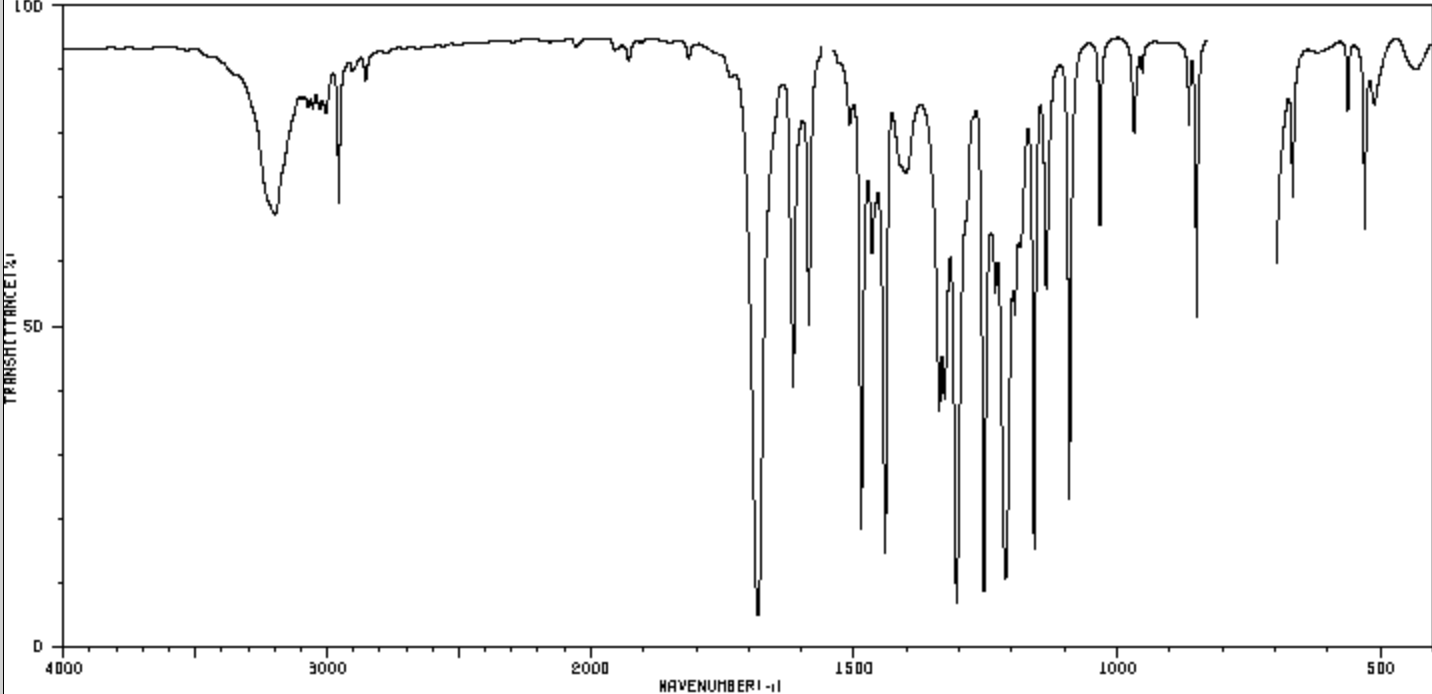
\includegraphics[width=\columnwidth]{database}
	\caption[billede]{IR-spektrum af methylsalicylat fra Japansk Database}
	\label{fig:database}
\end{figure}

Med det sagt, så kan vi fortsætte til vores IR-spektrum som ses på figur~\ref{fig:eksperiment}.

\begin{figure}[h!t]
	\centering
	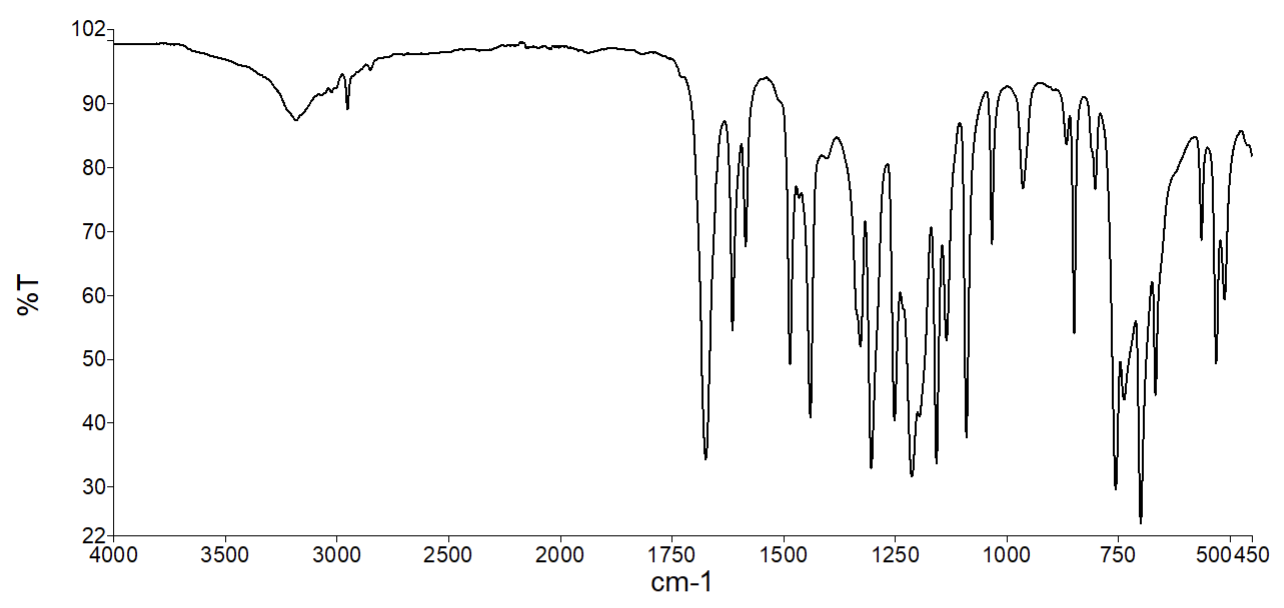
\includegraphics[width=\columnwidth]{eksperiment}
	\caption{IR-spektrum af synteseprodukt}
	\label{fig:eksperiment}
\end{figure}

Kaster man et hurtigt blik på figuren, så ligner de faktisk hinanden ret meget.
Dog kan man se, at udsvingene er væsentligt større på figur~\ref{fig:database},
hvilket giver rigtig god mening,
eftersom at vi pga.~vores "svovlsyre"\ nok ikke havde
en synderligt høj koncentration af methylsalicylat.
Man kan endda se, at vi har haft den forkerte katalysator, da 
$\ce{C-Cl}$ bindinger laver udslag v. $600-800\ \unit{\centi\meter^{-1}}$. Nu har figur~\ref{fig:database} ikke noget data i det interval,
men det er tydeligt i figur~\ref{fig:eksperiment},
at der er en vis mængde $\ce{C-Cl}$ bindinger.
